\documentclass[main.tex]{subfiles}
 
\begin{document}

\subsection{Urti elastici}

\textbf{Legame velocit\'a delle particelle CM-Lab}
Posto $\vec{r}=\vec{r_1}-\vec{r_2}$ vettore che separa le due particelle  e $\vec{v}=\dvec{r}=\dvec{r_1}-\dvec{r_2}$ velocit\'a relativa, nel sistema CM: $m_1\vec{r_1}+m_2\vec{r_2}=0$ quindi \lbt{\vec{r_{10}}=\frac{m_2}{m_1+m_2}\vec{r}}{\vec{r_{20}}=-\frac{m_1}{m_1+m_2}\vec{r}} e derivando rispetto a t ho le relazioni per le velocit\'a nel sistema CM \lbt{\vec{v'_{10}}=\frac{m_2}{m_1+m_2}\vec{v}}{\vec{v'_{20}}=-\frac{m_1}{m_1+m_2}\vec{v}} per tornare al Lab aggiungo la velocit\'a del centro di massa $\vec{V}=\frac{m_1\vec{v_1}+m_2\vec{v_2}}{m_1+m_2}$: \lbt{\vec{v_1}=\frac{m_2}{m_1+m_2}\vec{v}+\vec{V}}{\vec{v_2}=-\frac{m_1}{m_1+m_2}\vec{v}+\vec{V}}.

\textbf{Dopo l'urto}.

Gli impulsi restano uguali in modulo e opposti in verso; sia $\vec{n_0}$ la direzione di propagazione della particella di massa $m_1$, determinato dalla legge di interazione fra le due particelle, scrivo le velocit\'a delle 2 particelle dopo l'urto:

\lbt{\vec{v'_{10}}=\frac{m_2}{m_1+m_2}v\vec{n_0}}{\vec{v'_{20}}=-\frac{m_1}{m_1+m_2}v\vec{n_0}}.

Considero:

\lbt{\vec{p'_1}=m_1\vec{v'_1}=mv\vec{n_0}+\frac{m_1}{m_1+m_2}(\vec{p_1}+\vec{p_2})}{\vec{p'_2}=m_1\vec{v'_2}=-mv\vec{n_0}+\frac{m_2}{m_1+m_2}(\vec{p_1}+\vec{p_2})}, fissati gli impulsi iniziali, $\vec{p_1}$ e $\vec{p_2}$, gli impulsi dopo l'urto, $\vec{p'_1}=\vec{AC}$ e $\vec{p'_2}=\vec{CB}$, risultano dalla somma vettoriale dei fissi $\vec{AO}=\frac{m_1}{m_1+m_2}(\vec{p_1}+\vec{p_2})$ e $\vec{OB}=\frac{m_2}{m_1+m_2}(\vec{p_1}+\vec{p_2})$ con il vettore $\vec{OC}=mv\vec{n_0}$ con C che pu\'o assumere una posiione qualsiasi sulla circonferenza (composizione con i segni giusti).\\

Urto di 2 particelle: interpretazione geometrica

\includegraphics[scale=0.5]{scatteringmv12}
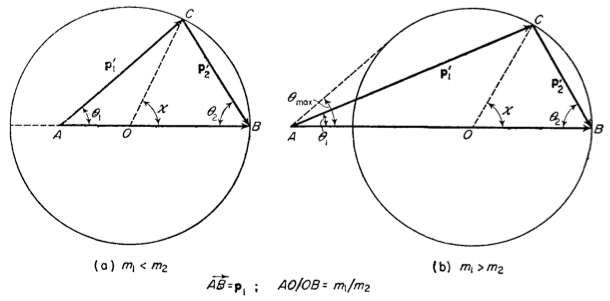
\includegraphics[scale=0.5]{scatteringmv1}
\includegraphics[scale=0.5]{m1eqm2}
Se la particella di massa $m_2$ \'e in quiete $v_2=0$:
\begin{itemize}
\item $\vec{OB}$ coincide con il raggio, $OB=\frac{m_2}{m_1+m_2}p_1=\frac{m_2m_1}{m_1+m_2}v_1=mv$
\item $\vec{AB}=\vec{AO}+\vec{OB}=\vec{p_1}$
\end{itemize}
Inoltre $OA=\frac{m_1}{m_1+m_2}(p_1)$: \lbt{m_2>m_1: OA<OC}{m_2<m_1: OA>OC}. Gli angoli $\theta_1$ e $\theta_2$ sono gli angoli di deflessione delle particelle dopo l'urto rispetto alla direzione di $\vec{p_1}$; l'angolo al centro $\chi$ \'e l'angolo di deviazione della particella incidente nel sistema CM.\\

\textbf{Masse uguali}
\lbt{\theta_1=\frac{\chi}{2}}{\theta_2=\frac{\pi-\chi}{2}}, \lbt{v'_1=v\cos{\frac{\chi}{2}}}{v'_2=v\sin{\frac{\chi}{2}}



Esprimo gli \textbf{angoli $\theta_1$ e $\theta_2$}  in funzione di $\chi$:\\
\lbt{\tan{\theta_1}=\frac{m_2\sin{\chi}}{m_1+m_2\cos{\chi}}}{\theta_2=\frac{\pi-\chi}{2}} e le \textbf{ velocit\'a dopo l'urto,$v'_1$ e $v'_2$} in funzione di $\chi$:\\
\lbt{v'_1=\frac{\sqrt{m_1^2+m_2^2+2m_1m_2\cos{\chi}}v}{m_1+m_2}}{v'_2=\frac{2m_1v}{m_1+m_2}\sin{\frac{\chi}{2}}}\\ $\theta_1+\theta_2$ \'e l'angolo formato dalle 2 direzioni lungo le quali le particelle si allontanano.
\textbf{Urto frontale}:\\
$\chi=\pi$: \lbt{\vec{v'_1}=\frac{m_1-m_2}{m_1+m_2}\vec{v}}{\vec{v'_1}=\frac{2m_1}{m_1+m_2}\vec{v}}, $\vec{v'_2}$ prende qui il massimo valore possibile quindi le'energia massima che la particella inizialmente in quiete pu\'o assumere \'e ${E_2}^{\text{Max}}=\frac{m_2{{v'_2}_{\text{max}}}^2}{2}=\frac{4m_1m_2}{(m_1+m_2)^2}$.\\
Nel caso $m_1>m_2$ ho un \textbf{angolo massimo di deflessione}: $\sin{\theta_{1\text{max}}}=\frac{m_2}{m_1}$.

\todo{Tikz:Disegno geometria scattering sfera impenetrabile}

\end{document}